\documentclass{article}
\usepackage[utf8]{inputenc}
\usepackage{graphicx}
\usepackage{amsmath}
\usepackage{hyperref}
\usepackage{geometry}
\usepackage{colortbl}
\usepackage{xcolor}
\usepackage{array}
\usepackage{booktabs}
\usepackage{authblk}
\usepackage{fancyhdr}
\geometry{a4paper}

\fancypagestyle{plain}{
    \fancyhf{}
    \renewcommand{\headrulewidth}{0pt}
    \renewcommand{\footrulewidth}{0pt}
    \fancyfoot[C]{\thepage}
}

\title{\huge{\textbf{Zcash: Advancing Privacy in Cryptocurrencies with zk-SNARK Technology}}}

\author[1]{Diana Decurti}
\author[2]{Fabrizio Emanuel}
\author[2]{Alberto Marino}
\author[2]{Michele Merico}
\author[2]{Michele Seira}

\affil[1]{\small Master’s degree student in Mathematics Engineering, Politecnico di Torino, Italy}
\affil[2]{\small Master’s degree student in Cybersecurity, Politecnico di Torino, Italy}
\date{\today}

\begin{document}

\pagenumbering{gobble}

\maketitle

\begin{center}
    \textit{Politecnico di Torino}
    
    \bigskip
    \textit{Blockchain and Cryptoeconomics Course (A.Y. 2023/2024)}
\end{center}

\begin{abstract}
\noindent The paper examines the Zcash cryptocurrency, which prioritizes user privacy through advanced cryptographic methods. Unlike typical cryptocurrencies, Zcash uses Zero-Knowledge Succinct Non-Interactive Argument of Knowledge (zk-SNARK) technology, enabling transaction verification without exposing private details. Launched on October 28, 2016, Zcash originated from the Zerocoin project at Johns Hopkins University, aimed at addressing Bitcoin's privacy issues. Users can choose between transparent and shielded transactions, significantly enhancing privacy and security. The paper also discusses Zcash's applications, including limited use on the Dark Web for activities like money laundering and illegal purchases, compared to other cryptocurrencies such as Monero. The conclusion highlights Zcash's need for ongoing innovation to stay competitive in the privacy-focused cryptocurrency market.
\end{abstract}

\bigskip
\noindent \textbf{Keywords:} Zcash; Blockchain; zk-SNARK; Bitcoin

\bigskip
\noindent This work is licensed under a \href{https://creativecommons.org/licenses/by/4.0/}{Creative Commons Attribution 4.0 International License}.

\newpage

\tableofcontents

\newpage
\section{Introduction}
Zcash represents a particularly interesting and innovative cryptocurrency with a number of unique features that differentiate it from other virtual currencies currently in circulation. Unlike most cryptocurrencies, which publicly reveal full transaction history on a distributed ledger, Zcash offers significant added value in terms of confidentiality, enhancing user privacy through advanced cryptographic techniques.

\noindent Zcash is the first completely open source cryptocurrency that comprehensively protects transactional privacy. This is achieved through the use of \textbf{ZKP (Zero-Knowledge Proofs)} technology, which prevents the reconstruction of asset passages, keeping transactions anonymous.

\noindent The creation of Zcash is the result of the work of a team of security engineers who developed an open source platform based on a modified version of the code of \textbf{Bitcoin}. The team includes almost all the creators of the Zerocoin and Zerocash protocols, a combination of scientists, engineers and consultants with advanced skills in cryptography and computer security.

\noindent Zcash originated in 2013 as \textbf{Zerocoin}, a project initiated by a group of researchers at Johns Hopkins University, including Matthew Green, Ian Miers, Christina Garman and Aviel D. Rubin. The main goal was to address the lack of privacy in Bitcoin by developing a cryptographic extension that would allow completely anonymous transactions. Zerocoin, initially conceived as an enhancement for Bitcoin, evolved in 2014 into \textbf{Zerocash}, a stand-alone digital currency that hides not only the origin of transactions but also the amount transferred.

\noindent Zcash was officially launched on 28 October 2016, distinguished by its use of \textbf{zk-SNARK (Zero-Knowledge Succinct Non-Interactive Argument of Knowledge)}, a cryptographic technology that allows transactions to be verified without revealing private details such as the sender, recipient or amount. This innovation allows Zcash to offer a higher level of privacy than Bitcoin, as sensitive information remains encrypted and invisible even on a public blockchain.

\noindent A useful analogy to understand the difference between Bitcoin and Zcash is that between the HTTP and HTTPS protocols. While HTTP is a protocol with no security guarantees, HTTPS adds a layer of protection based on encryption. Similarly, Zcash enhances the security and anonymity of transactions on a blockchain architecture similar to that of Bitcoin.

\noindent Zcash users can choose the degree of transparency of their transactions, opting for transparent or protected transactions via zk-SNARK. Zcash also offers features such as \textit{display keys} and \textit{payment disclosure}, which allow transaction details to be revealed only when necessary.

\noindent Despite its advanced privacy capabilities, it has been observed that many users prefer transparent transactions, limiting the effectiveness of Zcash's privacy features. This trend highlights the need for further studies and improvements to the protocol to maximise the privacy benefits offered by Zcash.

\noindent For a more detailed view of the history of Zcash see Figure \ref{fig:timeline}, which illustrates key historical events such as the founding of Zcash in 2016, the activation of the Overwinter and Sapling protocols, and the first halving in 2020. The current roadmap, which looks ahead to 2024, includes supporting the features introduced in Zcash, researching a PoW-PoS hybrid consensus model, and developing products to foster Zcash adoption.

\begin{figure}[!ht]
    \centering
    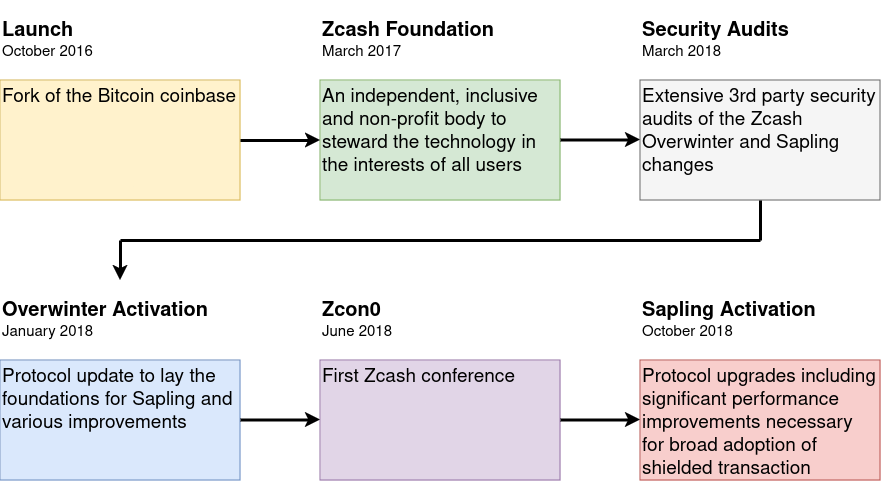
\includegraphics[width=1\linewidth]{img/timeline.png}
    \caption{Zcash Community History \cite{youtube}}
    \label{fig:timeline}
\end{figure}
\pagenumbering{arabic}
\section{Protocol}

The \textbf{blockchain} exploits the characteristics of a computer network of nodes (i.e. computers in the network with a copy of the blockchain ledger) and allows a ledger containing data and information to be managed and updated in an open, shared and distributed manner without the need for a central control and verification entity. Each blockchain is associated with a \textbf{protocol} that determines the structure of the blockchain and the way in which the blockchain handles transactions, defining its standards and modes of use.

\subsection{Zcash}

\noindent Unlike other blockchains, Zcash's blockchain allows transactions to be made, verified and recorded in two different ways: in \textbf{transparent} mode and in \textbf{shielded} mode. It is possible to distinguish the type of transaction by looking at the address prefix of the cryptocurrency involved.

\noindent Transparent addresses work like Bitcoin's, i.e. transaction data is public and visible on the blockchain. With shielded addresses, on the other hand, transactions take place without revealing the details of the transaction itself, such as the amount and addresses involved. 

\noindent In particular, there are three types of addresses, two of which are tied to their own value pool, which will henceforth be called \textbf{pool} for the sake of simplicity.

\noindent The \textbf{T} (transparent) addresses are bound to the only unshielded pool, also called the transparent pool. The transactions in this pool function like those in Bitcoin, not requiring any level of confidentiality by making each detail fully visible via a simple block explorer. As a result, it is possible to see the amount of the transaction, the starting address and the destination address.

\noindent On 28 October 2018, Zcash introduced the \textbf{Sapling} pool and \textbf{ZS} addresses, which use a ZKP (Zero-Knowledge Proof) called \textbf{zk-SNARK}. Using the Sapling pool, transaction details, such as amounts and addresses involved, are encrypted using the algorithm developed for Zcash, zk-SNARK, thus ensuring a high level of privacy and anonymity.

\noindent The Sapling pool uses a more secure and scalable version of the zk-SNARK algorithm used by the Sprout screen pool, identified with \textbf{ZC} addresses. This pool is now deprecated and no longer accessible.

\noindent On 31 May 2022, with the update called \textbf{NU5 (Network Upgrade 5)}, several new features were introduced, including \textbf{U} (unified) addresses. These types of addresses are different from addresses seen before, in that they are not linked to any particular pool, although it is a common misconception that they are linked to the \textbf{Orchard} pool, introduced with the same upgrade, NU5.

\noindent A unified address is a generic address that may contain various internal elements, known as \textbf{receivers}. This means that it can include receivers from different pools, thus allowing the customisation of one's U-address according to one's needs.

\noindent For example, we can create an address with a mix of receivers from the Transparent + Sapling + Orchard pool, Sapling + Orchard, or any other combination of pools. This offers maximum flexibility in managing one's U-address.

\noindent Another important feature of unified addresses is that they could theoretically offer the possibility of creating \textbf{multiasset} addresses, i.e. addresses that allow one to send and receive not only ZECs but also other assets, similar to Ethereum with ERC-20 tokens. This means that in the future they could be used as a platform for exchanging private digital assets, allowing parties to exchange assets without revealing transaction details.

\subsection{Verification of transactions and zk-SNARK technology}

On each blockchain, the information entered must be verified. Again, each blockchain decides how to verify this information. \textbf{Non-interactive zero-knowledge proofs} can be used in situations where there is no possibility of interaction between the demonstrator and verifier, such as in online transactions where the two parties are unable to communicate in real time. This makes non-interactive zero-knowledge proofs particularly useful in decentralised systems such as blockchains, where transactions are verified by a network of nodes and there is no central authority overseeing the verification process. Most non-interactive zero-knowledge proofs are based on mathematical constructs such as elliptic curve cryptography or coupling-based cryptography, which allow the creation of short and easily verifiable proofs of the truth of a statement. Non-interactive zero-knowledge proofs are designed to be efficient and can be used to verify a large number of statements simultaneously. To verify that transactions are correct on the blockchain, Zcash uses \textbf{zk-SNARK}, a particularly fast non-interactive zero-knowledge cryptographic proof.

\subsubsection{What is zk-SNARK}

\textbf{zk-SNARK} stands for \textbf{Zero-Knowledge Succinct Non-Interactive Argument of Knowledge} and is a type of cryptographic proof designed to guarantee the highest possible privacy. It is constructed using zero-knowledge protocols or tests (\textbf{ZKP, Zero-Knowledge Proof}), i.e. techniques that allow information to be validated and verified without having access to the information itself.

\noindent The abbreviation zk-SNARK contains the explanation of the proof itself:
\begin{itemize}
    \item \textbf{zk (Zero-Knowledge)}: a type of cryptographic proof that guarantees the confidentiality of information between users without compromising their security;
    \item \textbf{S (Succinct)}: refers to the brevity and speed with which evidence can be verified as true or legitimate. As this evidence proves the possession of information or data, its size is small, allowing it to be verified and validated in milliseconds;
    \item \textbf{N (Non-Interactive)}: indicates the absence of constant interaction between the demonstrator and the verifier. In zero-knowledge tests, it is sufficient to send a single message containing the proof to prove possession of the information, without the need for continuous or frequent communication between the parties;
    \item \textbf{ARK (Argument of Knowledge)}: refers to a proof of knowledge that the demonstrator can provide to the verifier to convince him of the possession of correct information, without revealing its content.
\end{itemize}

\noindent Basically, a zk-SNARK makes it possible to prove to a third party that you possess secret information without having to reveal it. At the same time, it provides irrefutable proof of the truthfulness of that claim. 

\subsubsection{The workings of zk-SNARK and Ali Baba's Cave of a Thousand Wonders}

The technology behind zk-SNARK is extremely complex and innovative. Its foundations were designed by cryptographers Shafi Goldwasser, Silvio Micali and Charles Rackoff in 1985. This technology makes it possible to prove knowledge of a secret without revealing it.

\noindent An explanatory example proposed by cryptographer Jean-Jacques Quisquater in 1990 may be useful to illustrate how ZKPs work.

\noindent The concept of ZKP is illustrated by means of a parabola involving the \textbf{The Cave of a Thousand Wonders of Ali Baba} (Figure \ref{fig:alibaba}).

\begin{figure}[!ht]
    \centering
    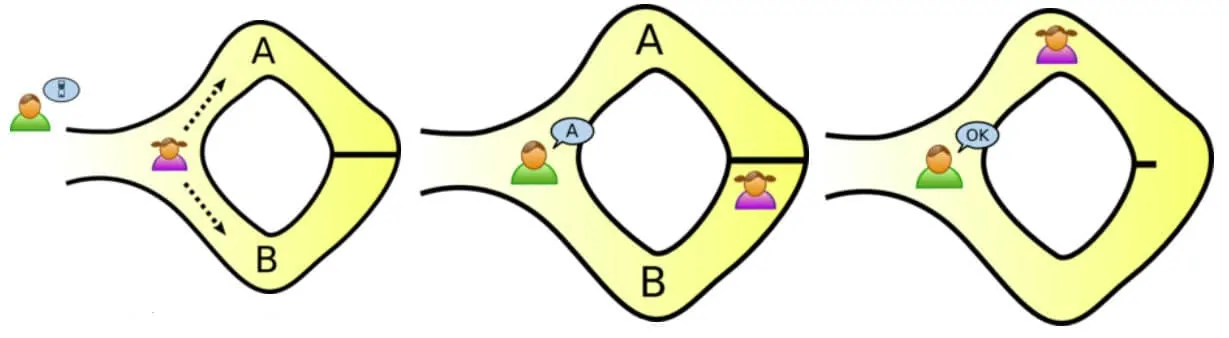
\includegraphics[width=1\linewidth]{img/alibaba.png}
    \caption{Example of Ali Baba's Cave of a Thousand Wonders}
    \label{fig:alibaba}
\end{figure}

\noindent Imagine a cave in the shape of a perfect circle, with a single entrance on the outside (the main entrance) and two paths leading to the same inner location, called the meeting point. Let these two paths be called path A and path B. Inside the cave, there is a small magic door that can only be opened by uttering the correct secret words.

\noindent Alice knows the secret words that open the magic door, while Bob wants to verify that Alice knows the secret words, but does not want Alice to reveal them to him.

\noindent How does the Zero-Knowledge Proof work?
\begin{enumerate}
    \item \textbf{Initial Position}: Alice enters the cave and chooses one of the two paths (A or B) without Bob seeing which one. She reaches the meeting point inside the cave and positions herself behind the magic door;
    \item \textbf{Bob's Choice}: Bob stands at the main entrance of the cave. From there, he calls out to Alice to come out from one of the two paths, A or B;
    \item \textbf{Alice's Response}: if Alice really knows the secret words, she can always open the magic door and exit from the path indicated by Bob. If Bob says "Path A," Alice opens the door and goes back through path A; if Bob says "Path B," Alice does the same but through path B;
    \item \textbf{Repetition of the Proof}: this process is repeated many times to reduce the probability that Alice is simply guessing the correct path. Each time, Alice randomly chooses a path (A or B) and Bob randomly asks for one of the two. After many iterations, if Alice is always able to exit from the requested path, Bob can be sure that Alice knows the secret words, as the probability that Alice correctly guesses each time becomes extremely low.
\end{enumerate}

\noindent Why is this considered a Zero-Knowledge Proof? There are essentially two reasons:
\begin{enumerate}
    \item \textbf{The secret is not revealed}: Bob never learns the secret words; he only verifies that Alice can open the magic door at any time;
    \item \textbf{Knowledge verification}: the repetition of the proof reduces the likelihood that Alice is simply guessing, convincingly demonstrating that she knows the secret words.
\end{enumerate}

\subsubsection{Importance of zk-SNARKs}

The ease with which transactions made by users can be tracked on public blockchains has led to the implementation of new security mechanisms to ensure that privacy is protected and maintained. This is essential for both users and cryptocurrencies, as privacy is a crucial element for the fungibility of digital currencies.

\noindent The implementation of privacy protocols, such as zk-SNARKs, makes it possible to guarantee the privacy of all users and participants in a blockchain network, without compromising the privacy or security of any of them. 

\noindent The use of zk-SNARKs can eliminate any kind of connection or relationship between the sender and the receiver, as well as the amounts involved in transactions. This security mechanism can be used in conjunction with other privacy technologies, such as Tor, which hides, for instance, the IP address of users. This makes privacy protection more effective in all transactions.

\subsection{Zcash and zk-SNARK}

\noindent The first cryptocurrency to apply zero-knowledge testing to ensure user privacy and security is Zcash (ZEC).

\noindent The choice to use zk-SNARK allows for a complete change in the way data is shared over the network, allowing transactions to remain encrypted while being verifiable and certifiable in terms of authenticity and validity. This offers an unprecedented level of anonymity, privacy, security and confidentiality for users.

\subsubsection{Zero Knowledge Protocol in Zcash}

The exceptional capability of the ZKP protocol to provide privacy enables the creation of an unprecedented secure communication system.

\noindent For all its properties, this privacy protocol has a wide variety of applications, ranging from military and national security implementations to secure communication and authentication systems, to cryptocurrencies and blockchain technology. In the latter field, ZKP protocols play a crucial role in protecting and maintaining the integrity of transactions conducted within the public blockchain, without revealing or leaking information among the parties involved. This is why Zcash has implemented the ZKP protocol in its system.

\subsubsection{Main features of Zcash thanks to zk-SNARK}

In Zcash, you can make transactions quickly, securely, and privately with low transaction fees of 0.0001 Zcash. Users have the option to use either fully private addresses or public and transparent addresses.

\noindent When using private addresses, information is not publicly disclosed, allowing users to include important information for the transaction recipient without exposing them to risks or vulnerabilities, as such information is protected and encrypted.

\noindent In cases where necessary, users can choose to disclose details of their transactions for auditing purposes or to comply with regulatory standards. However, the user retains full control over which transaction information they wish to reveal. Therefore, it is possible to display transferred amounts, addresses, or any related messages without revealing the identity of the sender or the recipient of the transaction.

\subsection{The elliptic curve of Zcash}

The elliptic curve of Zcash, named \textbf{Jubjub}, is a \textbf{Montgomery elliptic curve} used in cryptography for protecting sensitive data in the context of cryptocurrencies. It is designed to be efficient in both computation and cryptographic security, especially for use in zk-SNARKs.

\noindent Montgomery elliptic curves are similar to traditional elliptic curves but with a fundamental difference: the addition operation. In traditional elliptic curves, adding two points on the curve is a complex operation that requires several multiplications and inversions. In Montgomery elliptic curves, however, the addition can be performed with just one multiplication and one modular inversion. This simplification makes Montgomery elliptic curves much more efficient for cryptographic operations.

\noindent JubJub was developed by Daniel J. Bernstein and distinguishes itself from traditional elliptic curves with its notable advantages, including:

\begin{itemize}
    \item \textbf{Efficiency}: cryptographic operations performed on JubJub are faster and require less energy consumption compared to other curves;
    \item \textbf{Security}: JubJub is considered a robust elliptic curve resistant to known cryptographic attacks;
    \item \textbf{Compactness}: signatures and keys generated with JubJub are more compact than other curves, reducing transaction sizes and improving scalability.
\end{itemize}

\noindent The use of JubJub is a distinctive feature of Zcash and significantly contributes to its efficiency and privacy. The JubJub elliptic curve is employed for:

\begin{itemize}
    \item \textbf{Generating Z addresses}: Zcash addresses are anonymous and protect user privacy. JubJub is used to create these addresses securely and collision-resistant;
    \item \textbf{Encrypting transactions}: the values of Zcash transactions are encrypted to protect the confidentiality of the amounts sent. JubJub provides the mathematical basis for this encryption;
    \item \textbf{Generating anonymous signatures}: Zcash signatures allow users to spend their coins without revealing their identity. JubJub is used to create these signatures securely and anonymously.
\end{itemize}

\noindent In particular, the Montgomery curve (Figure \ref{fig:jubjub}), birationally equivalent to the JubJub curve, is defined by the equation:
\(y^2 = x^3 + 40962x^2 + x\)

\begin{figure}[!ht]
    \centering
    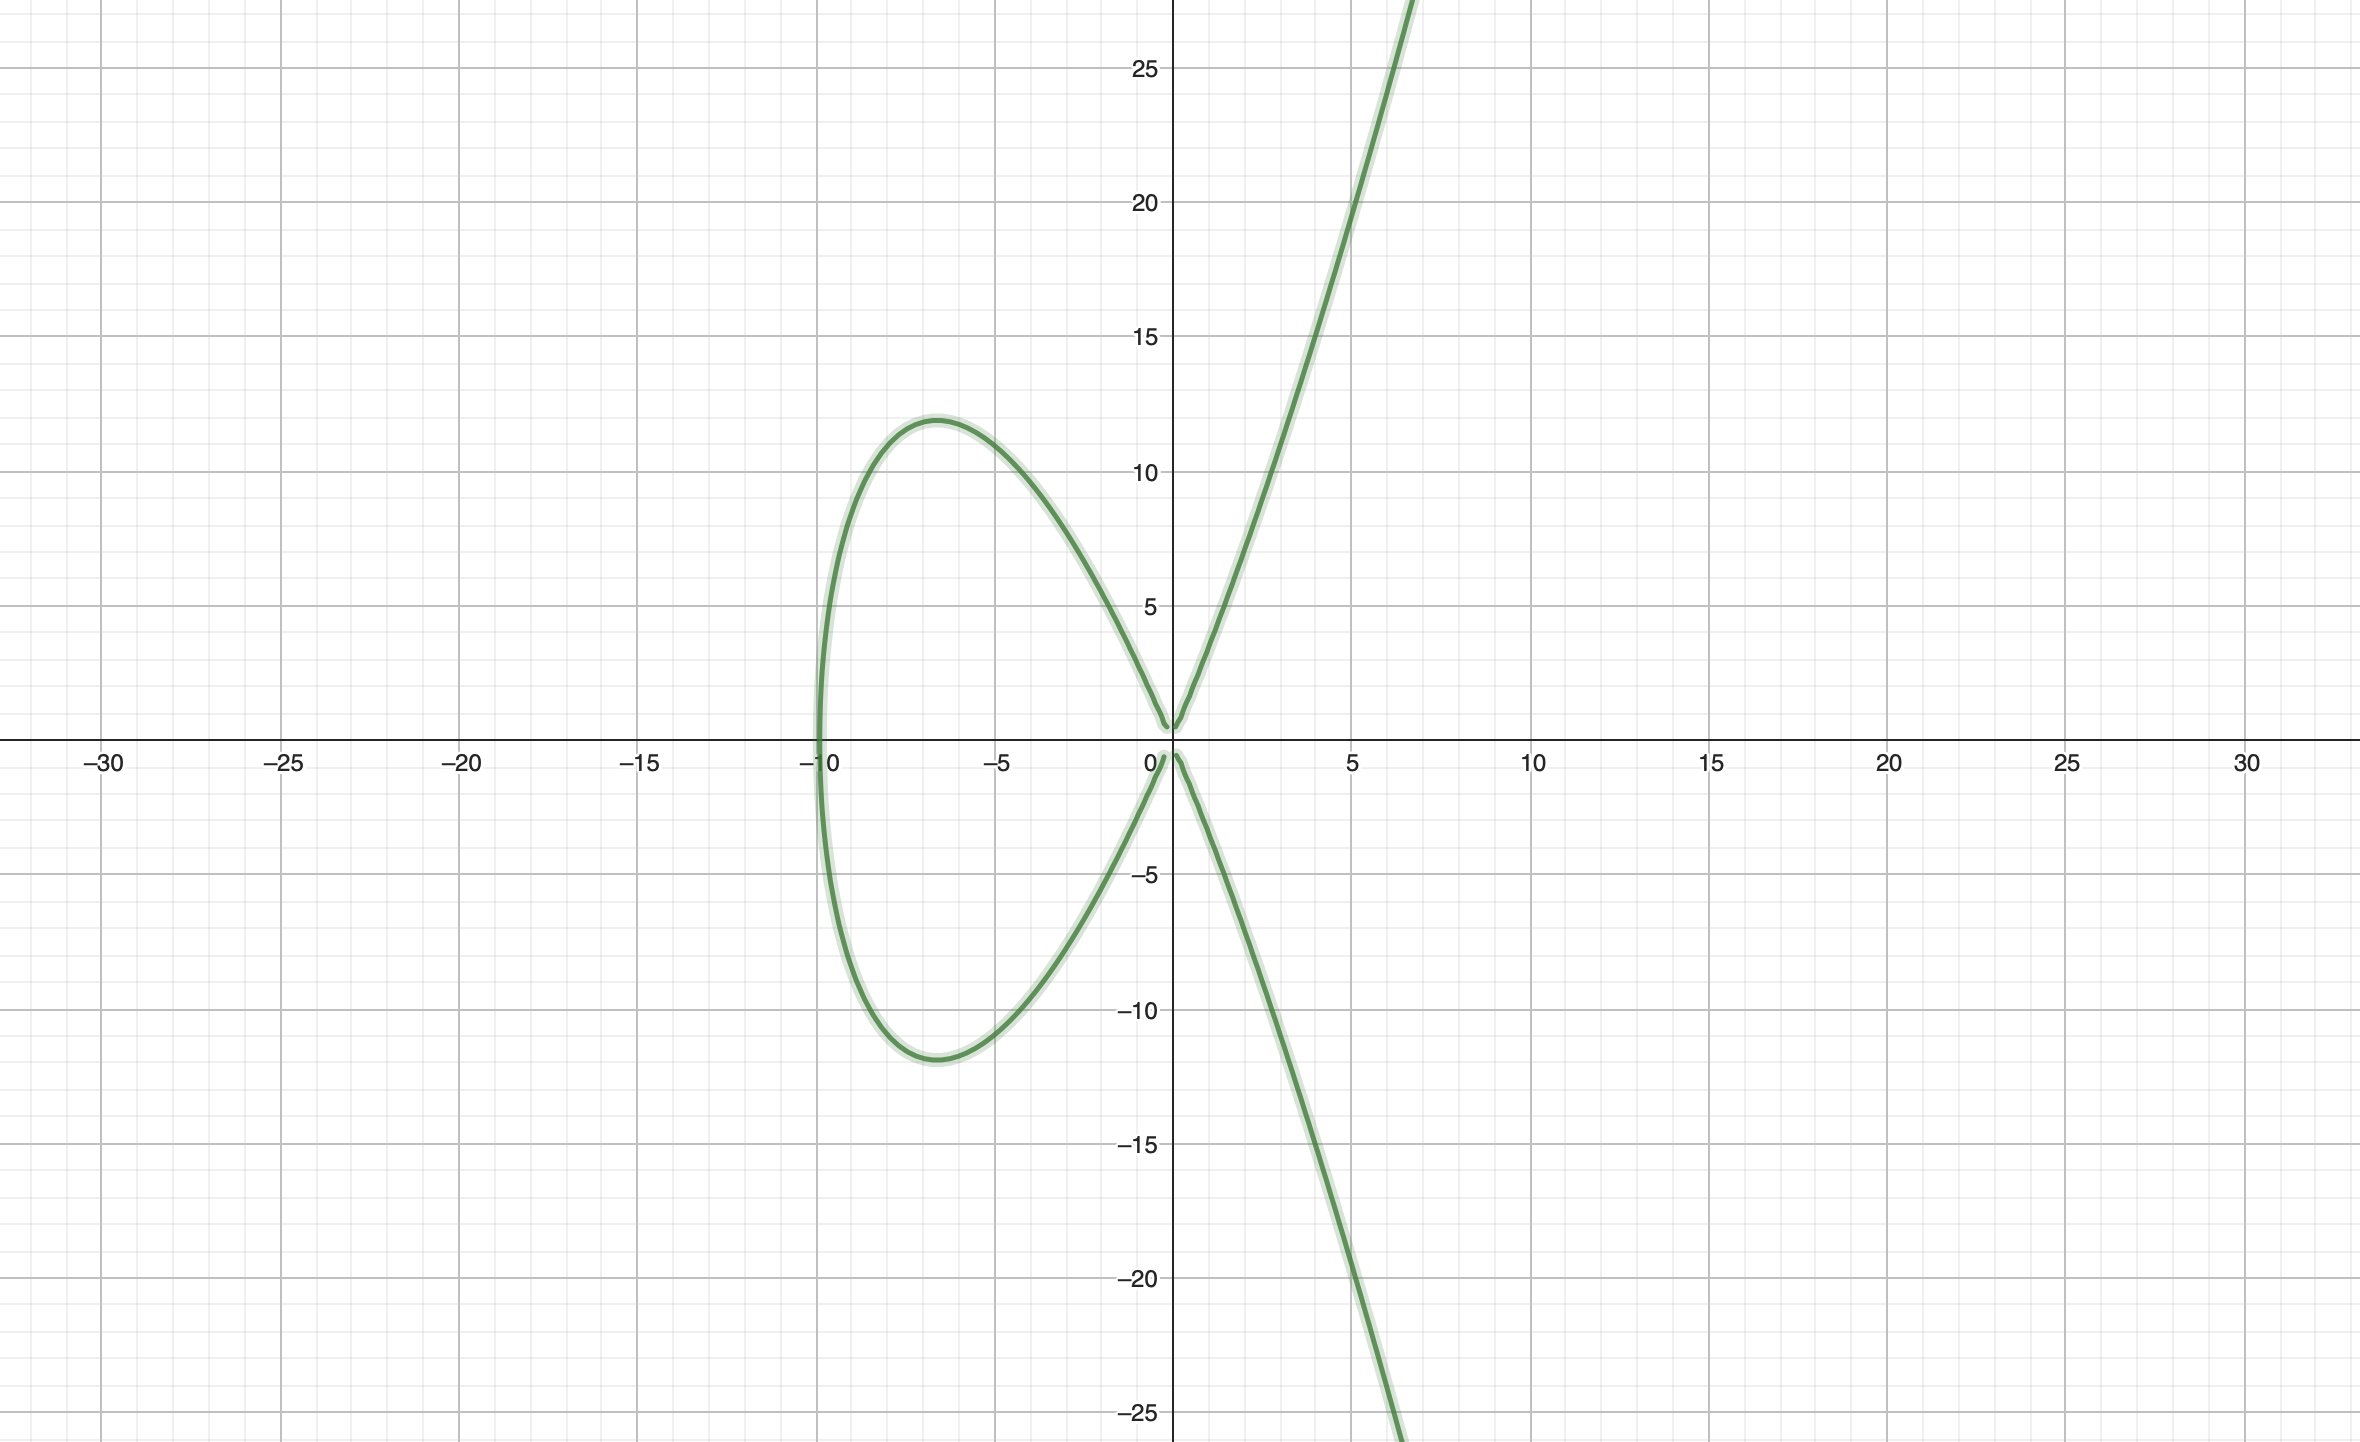
\includegraphics[width=1\linewidth]{img/jubjub.png}
    \caption{Elliptic Curve Montgomery}
    \label{fig:jubjub}
\end{figure}

\noindent Fundamentally, the JubJub elliptic curve represents a key component of Zcash technology and plays a crucial role in ensuring the privacy, security, and efficiency of transactions. Its selection represents a step forward compared to traditional elliptic curves and contributes to making Zcash one of the cryptocurrencies that most focus on user privacy.
\section{The Zcash Blockchain}

The first block of the Zcash blockchain is called the \textbf{genesis block} and has a height of 0. For each subsequent block, the height is incremented by 1. As in Bitcoin, at any given time, each miner is aware of a set of possible candidate blocks to enter the Zcash Blockchain. These form a tree rooted in the genesis block, where each node (block) refers to its parent through the \textbf{hashPrevBlock} field in the block header. To choose a possible new node among the candidates, a miner relies on the branch with the most work and selects that as the block to start generating a new block, referencing it in the hashPrevBlock.

\noindent Each block consists of the \textbf{header} and one or more \textbf{transactions}.

\subsection{Header}

The header consists of:
\begin{itemize}
    \item \textbf{nVersion}: this number indicates the rules to follow to validate a block; typically this value is 4;
    \item \textbf{hashPrevBlock}: this field contains the hash (SHA-256) of the previous block; this ensures that no previous block can be modified without also altering the header of this block;
    \item \textbf{hashMerkleRoot}: this value is derived from the hash (SHA-256) of \textbf{all} transactions in the block; thus, no transaction can be modified without changing this value;
    \item \textbf{hashReserved}: reserved field;
    \item \textbf{nTime}: the block's timestamp expressed in Unix epoch (UTC), indicating when the miner started hashing the header;
    \item \textbf{nBits}: as in Bitcoin, this number indicates the target threshold below which the header hash must fall; in other words, the header hash must be lower than this value;
    \item \textbf{nNonce}: an arbitrary field miners can change to alter the header hash to produce a hash equal to or below the target threshold;
    \item \textbf{solutionSize}: the size of an Equihash solution in bytes (always 1344);
    \item \textbf{solution}: the Equihash solution.
\end{itemize}

\subsection{Transactions}

Zcash transactions fall into two main categories:
\begin{enumerate}
    \item \textbf{Standard transactions}: these transactions are exactly like original Bitcoin transactions and maintain transparency;
    \item \textbf{Shielded transactions}: these transactions use zk-SNARK technology to enhance privacy.
\end{enumerate}

\noindent Shielded transactions represent an extension of the standard Bitcoin transaction structure, specifically designed to safeguard user privacy and protect financial activities from public scrutiny.

\noindent Transactions on Zcash can occur via two types of addresses:
\begin{itemize}
    \item \textbf{Shielded anonymous addresses (z-address)}: these addresses offer complete privacy. When both the sender and recipient use z-addresses, the entire transaction is shielded. This means the origin, destination, and amount of Zcash transferred are all hidden from public view on the blockchain;
    \item \textbf{Transparent addresses (t-address)}: these addresses function similarly to Bitcoin addresses. All transaction details are visible on the blockchain, analogous to traditional financial transactions.
\end{itemize}

\noindent When both parties in a Zcash transaction use z-addresses, zk-SNARK technology comes into play. zk-SNARK allows encrypting and verifying the transaction on the blockchain without revealing any sensitive details. This ensures the transaction's legitimacy while maintaining complete anonymity.

\begin{figure}[!ht]
    \centering
    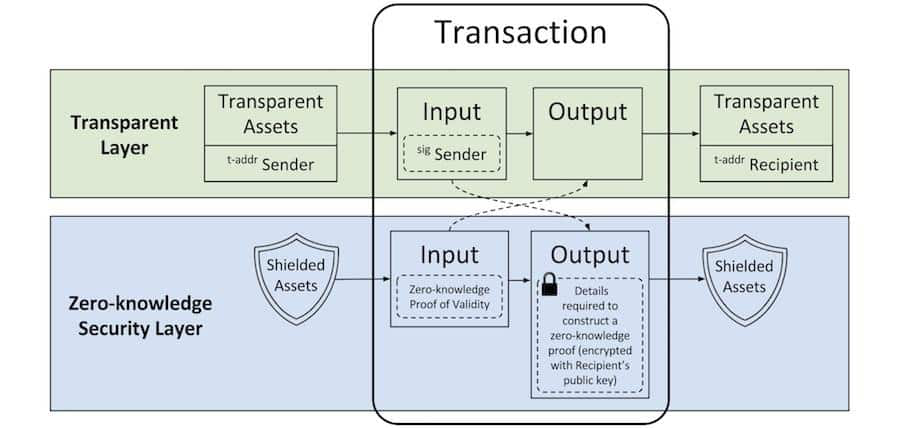
\includegraphics[width=1\linewidth]{img/zcashTransactions.png}
    \caption{Zcash Transaction}
    \label{fig:enter-label}
\end{figure}

\noindent In summary:
\begin{table}[!ht]
    \centering
    \begin{tabular}{>{\columncolor[gray]{0.9}}c|c|c}
        \toprule
        \rowcolor{gray!30}
        \textbf{Transaction Type} & \textbf{Privacy} & \textbf{Information Revealed} \\ \midrule
        Standard & Low & Sender, recipient, amount \\ \midrule
        Shielded & High & Sender, recipient, amount (hidden) \\ \bottomrule
    \end{tabular}
    \caption{Privacy levels of different transaction types}
    \label{tab:transaction_privacy}
\end{table}

\subsection{Sighash}

The \textbf{Sighash} is an essential component of the transaction signing mechanism in Zcash. It ensures that signed data has not been altered, protecting the transaction's integrity. It is a cryptographic hash calculated on specific elements of a transaction. This hash is then digitally signed to ensure the transaction cannot be modified without invalidating the signature.

\noindent The characteristics are as follows:
\begin{itemize}
    \item \textbf{Transaction structure}: as noted earlier, a Zcash transaction can contain multiple inputs, outputs, and, in the case of shielded transactions, zero-knowledge proofs;
    \item \textbf{Sighash calculation}: to create a signature, a hash (the sighash) of specific parts of the transaction is calculated. The digital signature is then created on this hash;
    \item \textbf{Types of Sighash}: Zcash inherits various types of sighash from Bitcoin, each with different implications for what is included in the hash calculation.
\end{itemize}

\noindent The sighash in shielded transactions must include the necessary elements to ensure critical data and zero-knowledge proofs have not been altered. The use of zk-SNARK proofs means that even the shielded parts of the transaction are included in the sighash calculation, ensuring private information is protected.

\noindent The different types of sighash are:
\begin{itemize}
    \item \textbf{SIGHASH-ALL}: signs the entire transaction. This is the most common type as it ensures no part of the transaction can be modified without invalidating the signature;
    \item \textbf{SIGHASH-NONE}: signs only the inputs, allowing modifications to the outputs without invalidating the signature. This type is less common as it offers less security;
    \item \textbf{SIGHASH-SINGLE}: signs only the corresponding input and output, allowing modifications to other inputs and outputs. Used in specific scenarios;
    \item \textbf{SIGHASH-ANYONECANPAY}: modifies the behavior of the previous sighashes by allowing anyone to add new inputs to the transaction without invalidating the original signature.
\end{itemize}

\noindent The hash algorithm used to calculate the sighash is the same as used by Bitcoin, i.e., SHA-256. More precisely, the hashing process involves a sequential double application of the algorithm, known as \textbf{double SHA-256}, to add an additional layer of security.

\noindent During the sighash calculation for a transaction, various fields of the transaction itself are included, such as inputs, outputs, and other metadata. The transaction is serialized, i.e., converted into a byte sequence, in a specific format. Only the fields necessary based on the sighash type (SIGHASH-ALL, SIGHASH-NONE, etc.) are included in the calculation. The hashing is then performed:
\begin{itemize}
    \item \textbf{First SHA-256}: the SHA-256 hash of the serialized data is calculated;
    \item \textbf{Second SHA-256}: the SHA-256 hash of the output of the first SHA-256 is calculated.
\end{itemize}

\noindent The resulting digest (sighash) is then digitally signed using the private key of the transaction's sender.
\section{Proof-of-Work}

Proof-of-Work (PoW) refers to any algorithm that operates on the concept of requiring a client to perform some work, which is then verified by the network. Typically, the required work involves performing complex calculations that are later verified by the network. These algorithms aim to discourage Denial of Service attacks and other abuses of service, such as network spam.

\subsection{Equihash}

Equihash is a Proof-of-Work (\textbf{PoW}) algorithm used by Zcash (formerly known as Zerocash) for mining. The Equihash algorithm was chosen for its features that promote decentralization and mining security, making this resource-intensive and costly process more accessible to everyone, while simultaneously making the currency more secure against centralized attacks.

\subsection{Details of the Equihash Algorithm}

Equihash is a PoW algorithm based on the generalized birthday problem, requiring a significant amount of memory to solve. Specifically:
\begin{itemize}
    \item \textbf{Birthday Paradox}: Equihash is based on a variant of this problem. It requires finding two distinct sets of nonces that, when used as input to a hash function, produce a result containing a specific sequence of leading zeros in the hash (similar to Bitcoin);
    \item \textbf{Parameters Used}: Equihash requires certain parameters to function correctly.
    \begin{itemize}
        \item \textbf{Parameter n}: This parameter defines the hash output size. In Zcash, the \textbf{Blake2b} hash algorithm is used to produce the hash output;
        \item \textbf{Parameter k}: This parameter affects the memory requirement to solve the problem; higher values of k correspond to greater memory demands and thus greater computational power required.
    \end{itemize}
\end{itemize}

\subsection{Mining Process with Equihash}

The term \textbf{mining} \cite{mining} can be translated as "extracting," emphasizing how it is a digital process through which cryptocurrencies can be obtained. Mining is not the creation of money through digital coins but a complicated verification procedure generated by leveraging the computing power of a computer or specialized tools designed for this purpose. Anyone providing computing power for mining operations becomes a \textbf{miner}. The mining process can be broken down into successive steps:
\begin{itemize}
    \item \textbf{Preparation}: The miner generates a block header that includes various information, such as a nonce and the Merkle Root of the transactions in the block;
    \item \textbf{Nonce Generation}: The miner varies the nonce and calculates hashes using Blake2b;
    \item \textbf{Solution Search}: The miner looks for pairs of nonces that meet the Equihash condition. Specifically, it seeks two distinct sets of nonces that, when combined, produce a hash with a specific number of leading zeros;
    \item \textbf{Verification}: The found solution must be easily verifiable but hard to find. This balances the algorithm, making mining fair for all participants;
    \item \textbf{Confirmation and Addition to the Block}: Once a valid solution is found, the block is added to the blockchain, and the miner receives a reward for the block.
\end{itemize}

\subsection{Miner Rewards}

Zcash miners are compensated for their work in verifying transactions and protecting the network through a combination of block rewards and transaction fees.
\begin{itemize}
    \item \textbf{Block Rewards}: Each new block created on the Zcash blockchain comes with a block reward, initially set at 2.0 ZEC. This reward has been gradually reduced over time following a halving schedule, similar to Bitcoin, to 0.625 ZEC (June 2024).
    These block rewards incentivize miners to contribute their computing power to the network. The rewards are distributed among all miners who contributed their computing power to the creation of a new block;
    \item \textbf{Transaction Fees}: Miners can also earn transaction fees from users sending Zcash transactions. These fees are voluntary and set by the transaction sender. However, a minimum fee is enforced to prevent an overwhelming number of transactions from being sent to the Zcash network merely to add (useless) work to the network.
\end{itemize}

\subsection{Advantages of Equihash}

The use of Equihash, while merely an implementation choice, brings several advantages to Zcash:
\begin{itemize}
    \item \textbf{ASIC Resistance}: By requiring a significant amount of memory, Equihash makes the use of ASICs (Application-Specific Integrated Circuits designed for a single specific use, such as mining a specific cryptocurrency) less advantageous compared to GPUs or CPUs, promoting more decentralized Zcash mining;
    \item \textbf{Security}: The nature of the birthday problem ensures that finding a valid solution requires a significant amount of calculations, guaranteeing the security of the network;
    \item \textbf{Decentralization}: By favoring the use of common hardware, Equihash helps maintain a more decentralized network compared to other PoW algorithms dominated by ASICs (e.g., Bitcoin).
\end{itemize}
\section{Uses of Zcash}

Zcash can be used as a speculative investment tool and/or as a form of payment. When used as a speculative investment tool, the actual profit from the investment can vary over time depending on the fluctuation of Zcash's price, as the cryptocurrency market is highly volatile. Nevertheless, the most interesting use is as a form of payment, as Zcash allows for transactions where amounts, recipients, and senders remain \textbf{anonymous}. This feature makes Zcash popular for payments on the \textbf{Dark Web}.

\subsection{Zcash on the Dark Web}

The Deep Web is everything that is not visible on search engines, while the Dark Web refers to Deep Web content accessible via the internet through specific software, configurations, and authorization. On the Dark Web, a vast amount of products and services, both legal and illegal, can be purchased.

\noindent Payments on the Dark Web are made with cryptocurrencies due to their decentralization and, most importantly, the privacy guarantees they offer. The most used cryptocurrencies on the Dark Web are Monero, Dash, Litecoin, Bitcoin (even though Bitcoin's privacy is not correctly guaranteed), but also Zcash itself.

\noindent According to research conducted by the RAND Corporation \cite{rand}, there is some \textbf{possible evidence} indicating that Zcash may be used for:
\begin{itemize}
    \item \textbf{Money laundering}: Zcash is particularly suitable for money laundering, as every single financial transaction is impossible to trace and identify;
    \item \textbf{Payments for purchasing illegal goods and services}: various studies show that Zcash is accepted as a form of payment on the Dark Web;
    \item \textbf{Terrorist financing}: it has been discovered that a Telegram account titled “Supporto tecnico della Fondazione Afaq Electronic Foundation,” a media group associated with ISIS, advised followers to use Zcash instead of Bitcoin for transactions directed to the group.
\end{itemize}

\noindent On the Dark Web, various e-commerce platforms sell diverse services and products. The most well-known is certainly \textbf{Dream}, but it is not the only one (Figure \ref{fig:e-commerce}). Many e-commerce platforms, such as the \textbf{Berlusconi} e-commerce, were later shut down, but they still marked an important gathering point for criminals for years.

\noindent The most sold services, goods, and products on various Dark Web e-commerce platforms are drugs, frauds, digital goods, but also weapons and jewelry.

\begin{figure}[!ht]
    \centering
    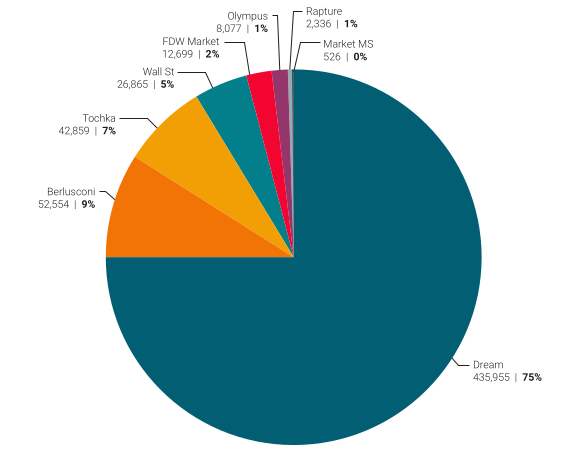
\includegraphics[width=1\linewidth]{img/eCommerce.png}
    \caption{E-commerce on the Dark Web}
    \label{fig:e-commerce}
\end{figure}

\noindent Multiple cryptocurrencies are used for purchases. The most used is Bitcoin, followed by Monero and Ethereum. Zcash is, along with Litecoin, one of the less used currencies for payments. A summary of the payment distribution is presented in Figure \ref{fig:cryptoPayments}.

\begin{figure}[!ht]
    \centering
    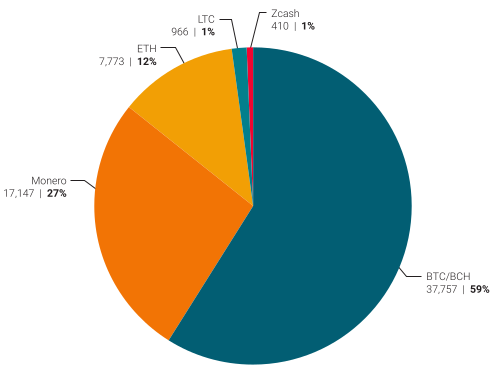
\includegraphics[width=1\linewidth]{img/cryptoPayments.png}
    \caption{Cryptocurrencies used for making payments}
    \label{fig:cryptoPayments}
\end{figure}

\noindent Further research indicates that Zcash is mentioned as an accepted payment form primarily by three sellers:
\begin{itemize}
    \item \textbf{TheShop};
    \item \textbf{Skyscraper};
    \item \textbf{Cyberzen}.
\end{itemize}

\noindent Although Zcash is potentially suitable for handling transactions related to the purchase of illegal goods and/or services, its use is still limited. The reason is simple: Zcash was created as a cryptocurrency that aims to ensure privacy, not to facilitate untraceable illegal payments, but to offer an additional form of protection to the end user in terms of traceability. Monero, for example, is a cryptocurrency created with the intent of becoming the most widespread form of payment on the Dark Web from the very beginning.

\noindent In conclusion, Zcash represents a significant evolution in the cryptocurrency landscape, combining blockchain security with transaction privacy.
\section{Conclusions}

In conclusion, Zcash represents a significant evolution in the cryptocurrency landscape, combining blockchain security with transaction privacy. Its advanced technology and focus on confidentiality offer new opportunities for a potentially safer and more transparent financial market.
The future looks promising, with numerous developments underway aimed at further improving its security, scalability, and usability \cite{zcash-future}. The Zcash community and its developers are working on significant updates, such as implementing transaction complexity reduction technologies and optimizing the network to handle a higher volume of transactions \cite{forum}.

\noindent However, despite its technical advantages, the mass adoption of Zcash remains a challenge. Many users and merchants are still more inclined to use more well-known cryptocurrencies like Bitcoin and Ethereum. Additionally, the anonymous nature of transactions might attract the attention of regulatory authorities, who could see this feature as a risk for money laundering and other illicit activities \cite{zcash-privacy}.

\noindent Finally, the field of privacy-oriented cryptocurrencies is competitive, with coins like Monero and Dash also offering advanced anonymity features. Zcash must continue to innovate to try to establish itself as a leader in the sector.

\newpage
\bibliographystyle{plain}
\bibliography{bibliography}

\end{document}
